\documentclass[10pt]{beamer}

\usetheme[progressbar=frametitle]{metropolis}
\usepackage{appendixnumberbeamer}
\usepackage{pdfpages}
\usepackage{booktabs}
\usepackage[scale=2]{ccicons}

\usepackage{pgfplots}
\usepgfplotslibrary{dateplot}

\usepackage{xspace}
\newcommand{\themename}{\textbf{\textsc{metropolis}}\xspace}

\usepackage{caption}
\captionsetup[figure]{labelformat=empty}

\usepackage{graphicx}

\title{A Benchmark Suite for Serverless Computing}
\subtitle{AWS Lambda - Microsoft Azure Functions -
\\Google Cloud Functions - IBM Cloud Functions \newline \newline Master Thesis - Final Presentation}
% \date{\today}
\date{March 2, 2020}
\author{Pascal Maissen\newline \href{mailto:pascal.maissen@unifr.ch}{pascal.maissen@unifr.ch}}
\institute{Swiss Joint Master of Science in Computer Science, University of Neuchâtel}
% \titlegraphic{\hfill
\includegraphics[height=1.5cm]{logo.pdf}}

% 25 + 5 min
% the main problem you tackled
% the proposed solution
% details of the implementation
% some of the results (not all) presented in the report
% small discussion of the results
% you could even make a 1 minute demo, if you feel brave :-)

\begin{document}

\maketitle

\begin{frame}{Table of contents}

	\begin{itemize}
		\item Problem Description and Motivation
		\item Serverless - Function as a Service (FaaS)
		\item Proposed solution
		\item Implementation
		\item Demo
		\item Results
		\item Summary and Discussion
	\end{itemize}
	
\end{frame}

\begin{frame}{Problem Description and Motivation}

	\begin{itemize}
		\item Trend towards cloud computing
		\item Many (smaller) businesses are not interested in managing and maintaining hardware, VMs or operating systems
		\item Solution: Serverless computing
		\item Focus on Function as a Service (Faas)
		\item Not much effort so far to test, benchmark and compare offered platforms
	\end{itemize}
	
	
\end{frame}

\begin{frame}{FaaS - Overview}
\begin{center}
\textbf{High-level serverless FaaS platform architecture}
\end{center}
\vspace{-1cm}
	\begin{figure}
	\centering
	%\caption{High-level serverless FaaS platform architecture}
	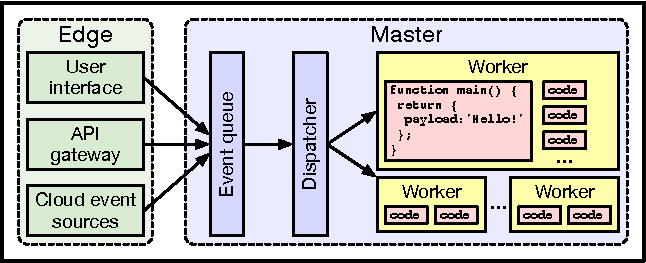
\includegraphics{bilder/FaaS}
	\end{figure}
	\vspace{-1cm}
	\begin{block}{}
		\linespread{0.8}\selectfont
	\scriptsize \textbf{Source:} Castro, Paul ; Ishakian, Vatche ; Muthusamy, Vinod ; Slominski, Aleksander:\\ The Rise of Serverless Computing. In: Commun. ACM 62 (2019), November, Nr. 12, 44–54. http://dx.doi.org/10.1145/3368454. – DOI 10.1145/3368454. – ISSN 0001–0782
	\end{block}
\end{frame}

\begin{frame}{FaaS - Characteristics}

	\begin{itemize}
		\item Stateless
		\item Automatic scaling
		\item No hardware and server management
		\item Paid per usage
		\item Usage: Application backends and data processing
	\end{itemize}
	

\end{frame}

\begin{frame}{FaaS - Challenges}

	\begin{itemize}
		\item Performance
		\item Scalability
		\item Usability
		\item Pricing
		\item Limitations
	\end{itemize}

\end{frame}

\begin{frame}{Proposed Solution}
\textbf{Benchmark suite for serverless computing}
	\begin{itemize}
		\item Packaged with Docker
		\item Easy to use
	\end{itemize}
	
	\vspace{0.5cm}
	
	\begin{columns}[T,onlytextwidth]
    \column{0.33\textwidth}
      \textbf{4 Clouds:}
      \begin{itemize}
        		\item AWS Lambda
			\item Azure Functions
			\item Google Functions
			\item IBM Functions
      \end{itemize}

    \column{0.4\textwidth}
      \textbf{4 Runtimes:}
      \begin{itemize}
        \item Node.js (JavaScript)
        \item Python
        \item Go
        \item .NET Core (\texttt{C\#})
      \end{itemize}

    \column{0.27\textwidth}
      \textbf{5 Tests:}
      \begin{itemize}
        \item Latency
        \item Factors (CPU)
        \item Matrix (CPU)
        \item File system
        \item Custom
      \end{itemize}
  \end{columns}
	
\end{frame}


{
\setbeamercolor{background canvas}{bg=white}
\begin{frame}{Implementation - Overview}

	\begin{figure}
	\centering
	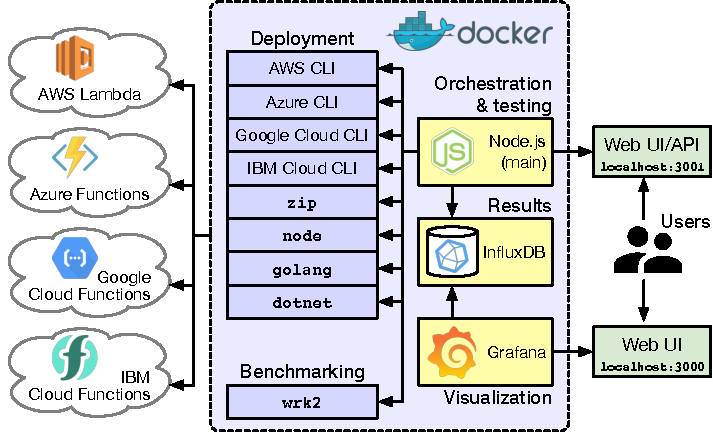
\includegraphics[scale=0.7]{bilder/archi}
	\end{figure}
	
\end{frame}
}

\begin{frame}{Implementation - Functionality}

\textbf{Main application:}
	\begin{itemize}
		\item Deployment and cleanup of tests
		\item Testing: Observer general performance and handling
		\item Benchmarking: Load test a function
		\item Pricing: Theoretical and practical
	\end{itemize}
\textbf{Results:}
\begin{itemize}
	\item Stored into InfluxDB
	\item Visualization in Grafana
\end{itemize}
\end{frame}

\begin{frame}[standout]

	Demo

\end{frame}

{
\setbeamercolor{background canvas}{bg=white}
\begin{frame}{Results - Cold Start}


\noindent\makebox[\textwidth]{%
  %\begin{figure}
	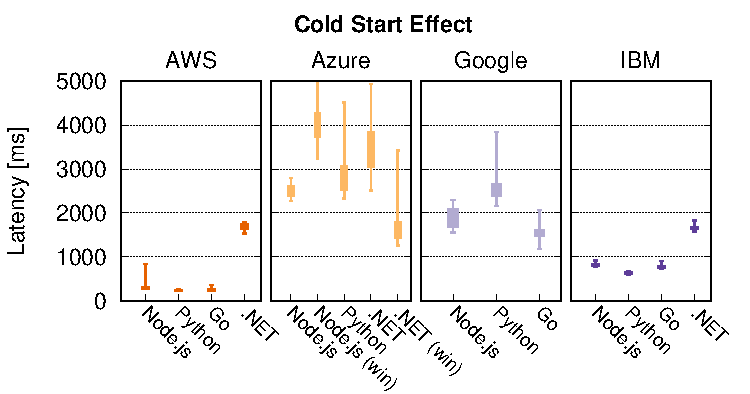
\includegraphics{bilder/coldstart_whisker}
	%\end{figure}	
}

	
\end{frame}
}

{
\setbeamercolor{background canvas}{bg=white}
\begin{frame}{Results - General Performance}

\noindent\makebox[\textwidth]{%
  %\begin{figure}
	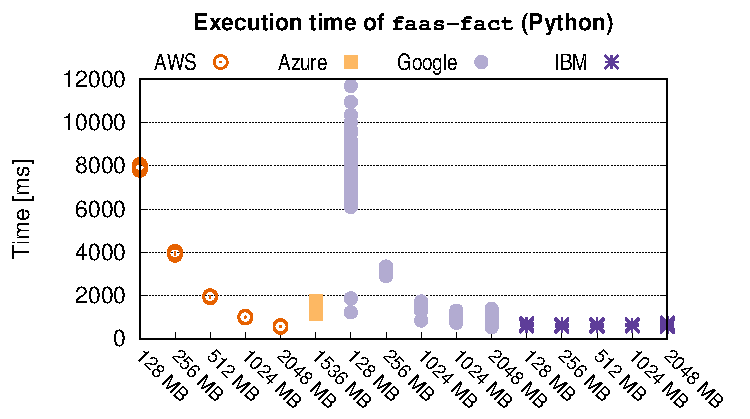
\includegraphics{bilder/cpufact}
	%\end{figure}	
}

\end{frame}
}

{
\setbeamercolor{background canvas}{bg=white}
\begin{frame}{Results - Load Test (Average Latency)}

	\noindent\makebox[\textwidth]{%
	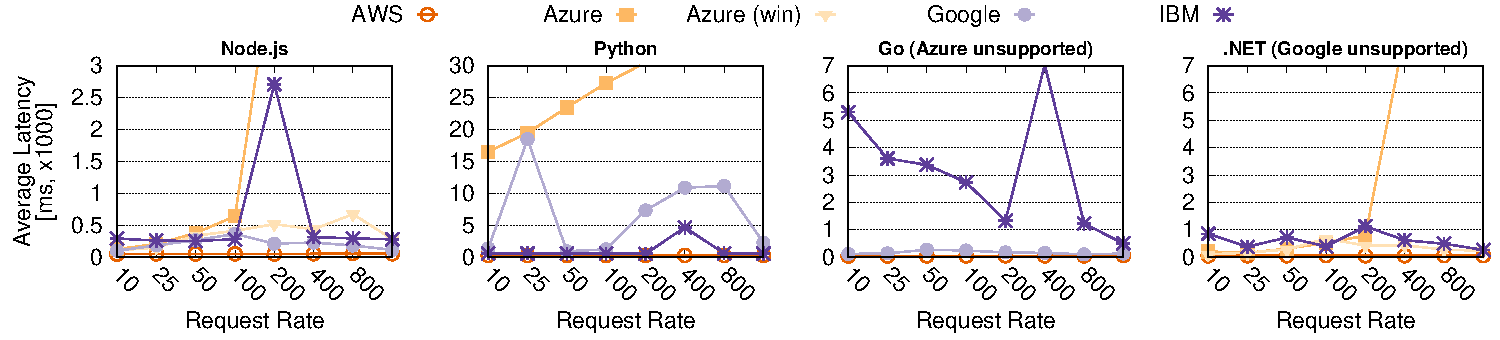
\includegraphics[scale=0.5]{bilder/tputlat_combined}
	}
	
\end{frame}
}

{
\setbeamercolor{background canvas}{bg=white}
\begin{frame}{Results - Load Test (Percentiles)}

	\noindent\makebox[\textwidth]{%
	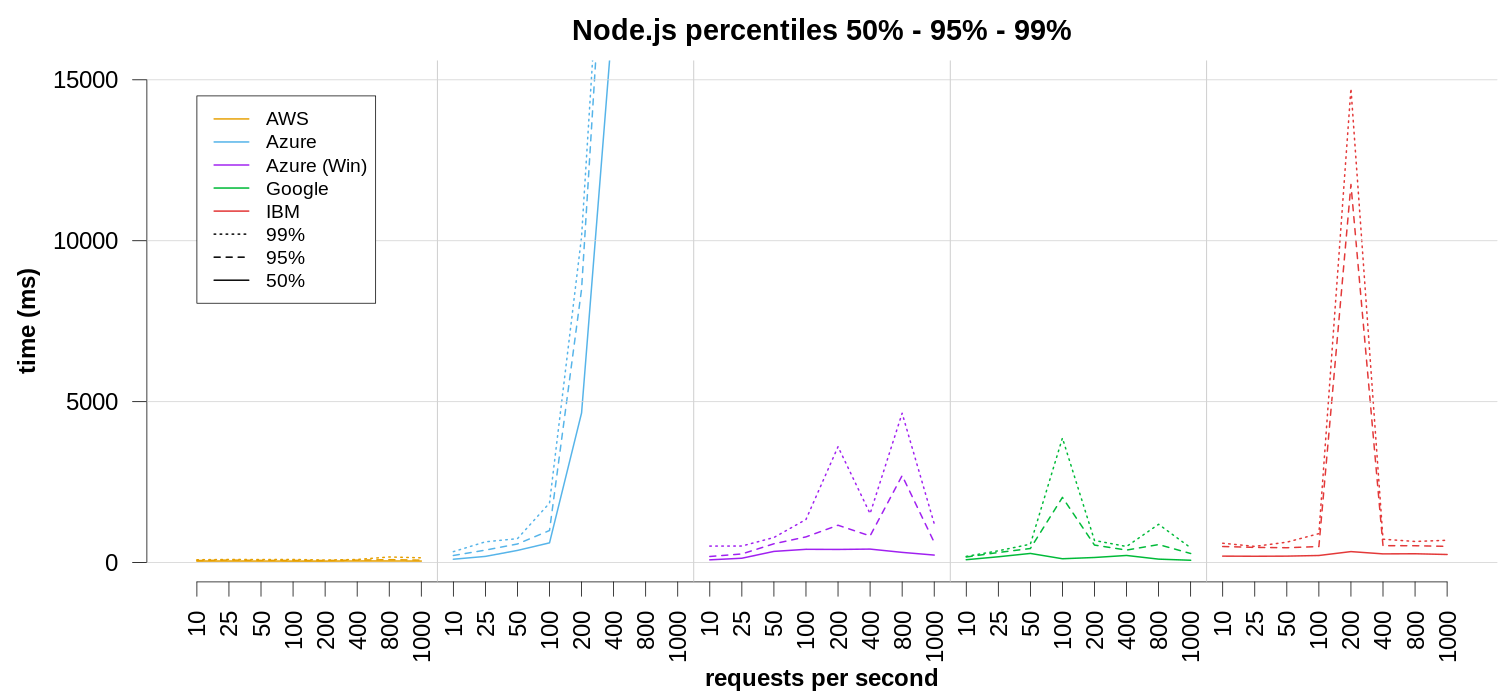
\includegraphics[scale=0.22]{bilder/plot_percentile_latency_node.png}
	}
	
\end{frame}
}

\begin{frame}{Future Work}

	\begin{itemize}
		\item General optimizations and improvements
		\item Plotting integration (e.g. R)
		\item Continuous deployment
		\item More detailed load test
		\item Real world application benchmark
		\item Test docker images instead of given runtimes
	\end{itemize}

\end{frame}

\begin{frame}{Summary and Discussion}

	\begin{itemize}
		\item[] \textbf{Testing:} Important to test and optimize the code
			\begin{itemize}
				\item Execution time
				\item Memory needed
				\item Save costs
			\end{itemize}
		\item[] \textbf{Scaling:} Test a scenario as close as possible to the actual load. Clouds and runtimes can differ a lot in scaling.
		\item[] \textbf{Pricing:} Estimate prices according to test results and not just using the offered pricing calculator
		\item[] \textbf{No standard:} There is no standard framework between the clouds
	\end{itemize}

	\textbf{Serverless can be a valid option depending on the workload and the requirements. This suite helps with the analysis and the decision.}

\end{frame}

\end{document}
